\section{Sterna}
  \paragraph{}
    Sterna is an addon to Blender, a 3D modeling software. Sterna allows the user to design, edit and visualize RNA strands.
\subsection{Basics}
  \subsubsection{Setup}
    To install Sterna:
    \verb+Navigate File -> Preferences -> Add-ons+. Select User category.
    If an older version of Sterna is already installed, deactivate it and remove it.
    Select Install Add-on from File. Find and select Sterna.zip.
    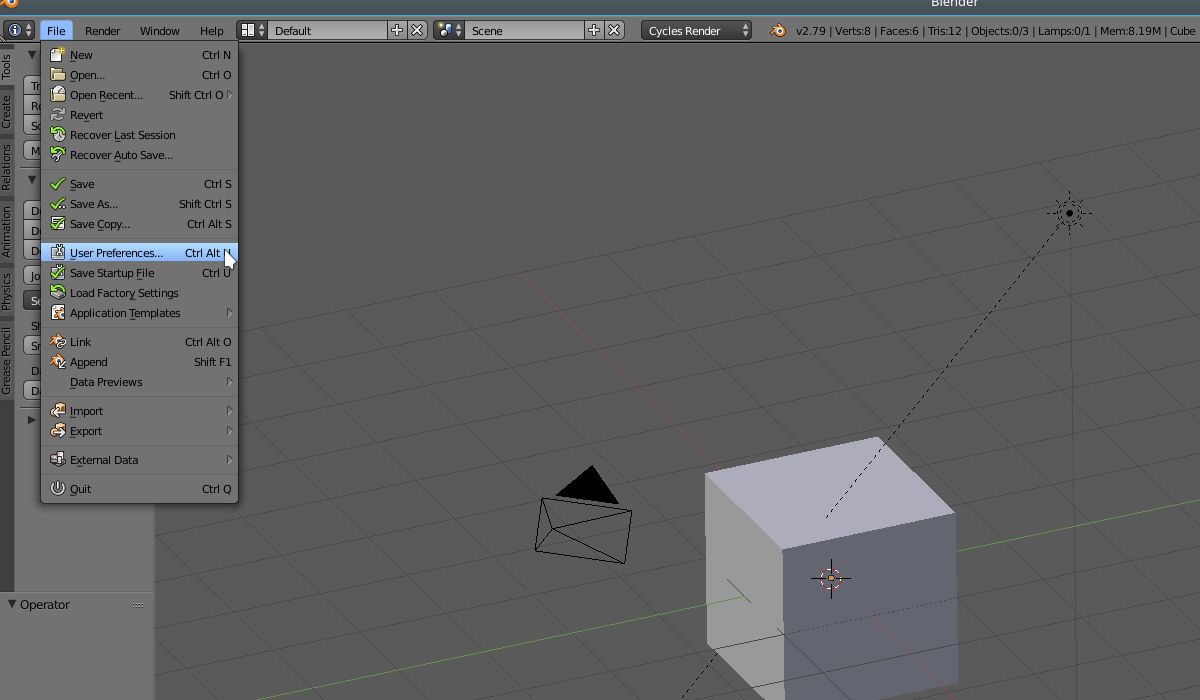
\includegraphics[width=\textwidth]{images/Sterna_1}
    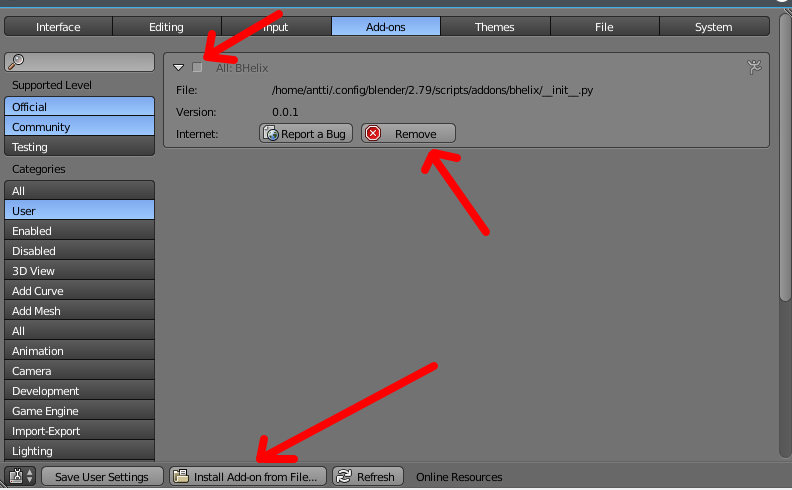
\includegraphics[width=\textwidth]{images/Sterna_2}
    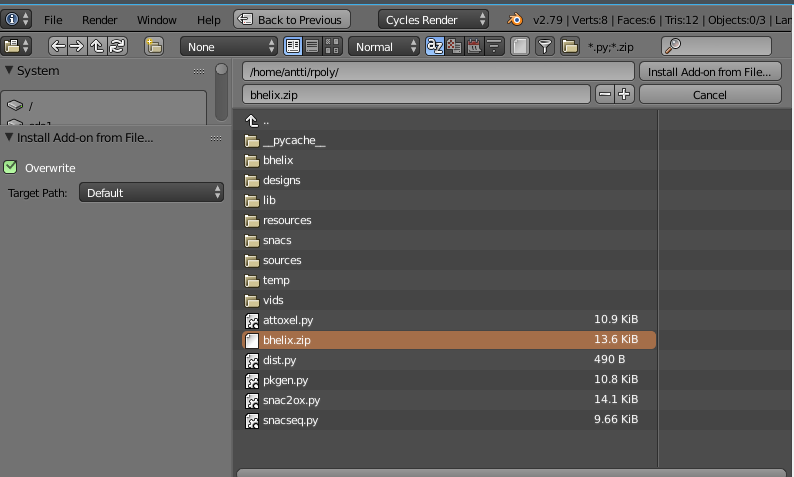
\includegraphics[width=\textwidth]{images/Sterna_3}
  \subsubsection{Use}
    The first step of designing an RNA strand is to choose a model. Any model will work as long as all its vertices are connected. To generate a helix:
    If you wish to choose the spanning tree edges, navigate to Data-tab and create a new edge group.
    Choose the object you wish to convert to a strand and go to edit mode by pressing TAB.
    Change the selection mode to edge-select by pressing CTRL + TAB.
    Select the edges and press assign button under the edge group.

    Next, navigate to the modifiers tab. If you wish to use a random spanning tree, tick "Use random spanning tree" box.
    By default, one blender unit is equal to 1 nm. This can be changed by modifying the scale parameter. The scale parameters defines how many nanometers each blender unit is. If the scale is too small, Sterna will be unable to fit a strand around the model.
    If you wish the edges to have integer number of turns, tick "Try to force integer number of turns", and select a number. This changes the scale in such a way that the edges of the object contain an integer multiple of 11 bases, which is the wavelength of an RNA helix. The results might be unsatisfactory for asymmetrical structures.
    Finally, click "Generate Helix" button to generate the RNA strand. If unsuccessful, try tweaking the parameters or the object. Usually a failure is due to too small a scale or faulty object. If tweaking the scale does not help, make sure the object has no disconnected components and that its normal vectors are properly defined.
    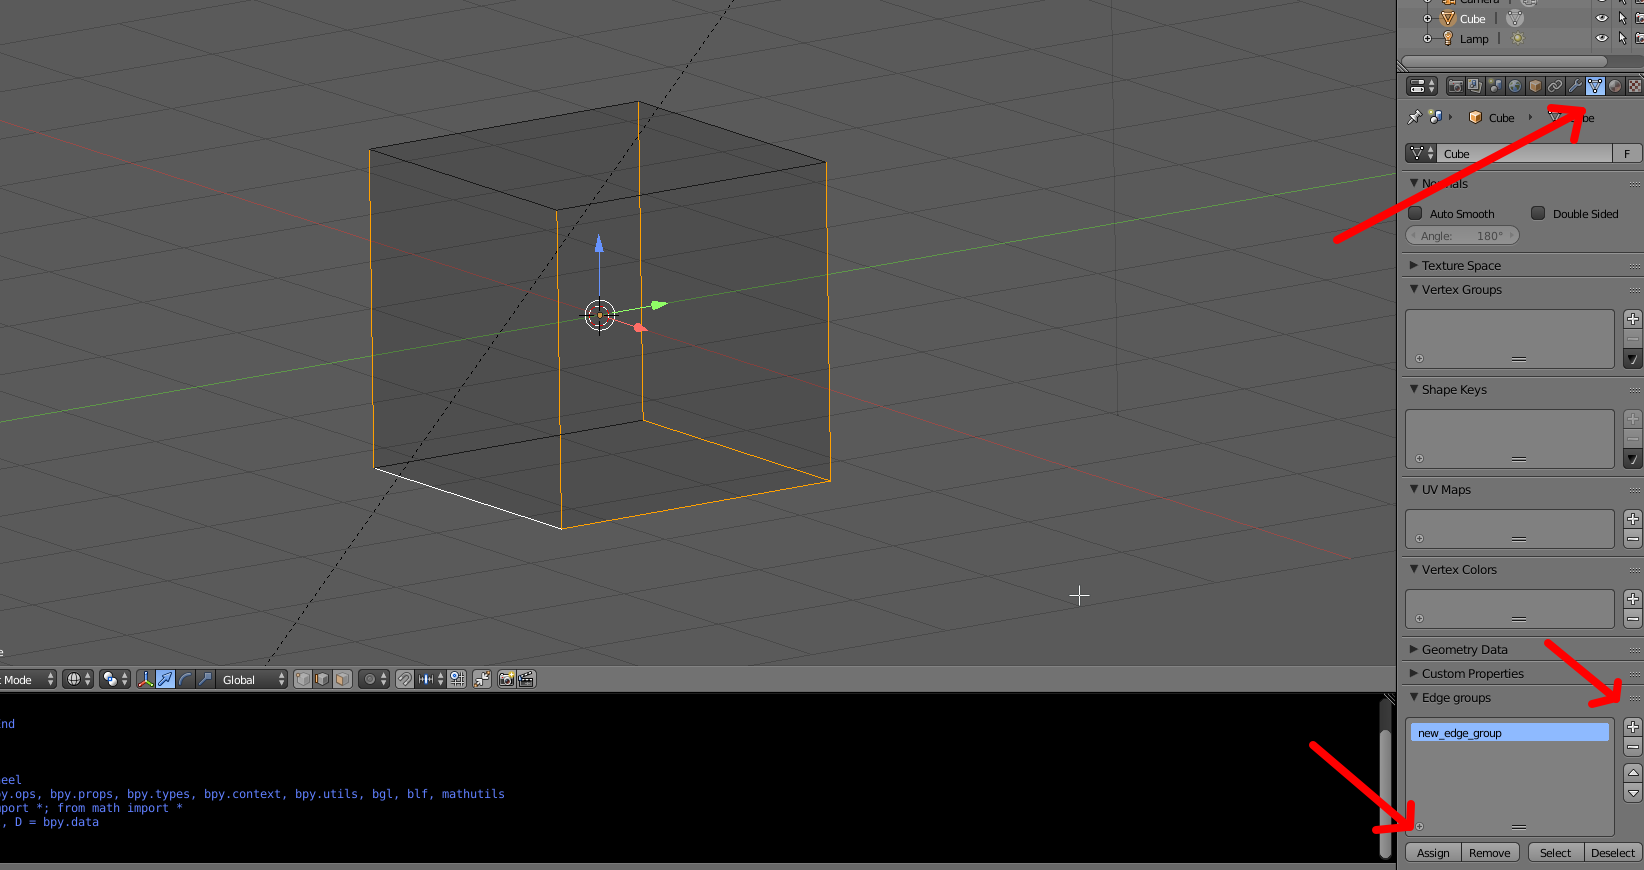
\includegraphics[width=\textwidth]{images/Sterna_4}
    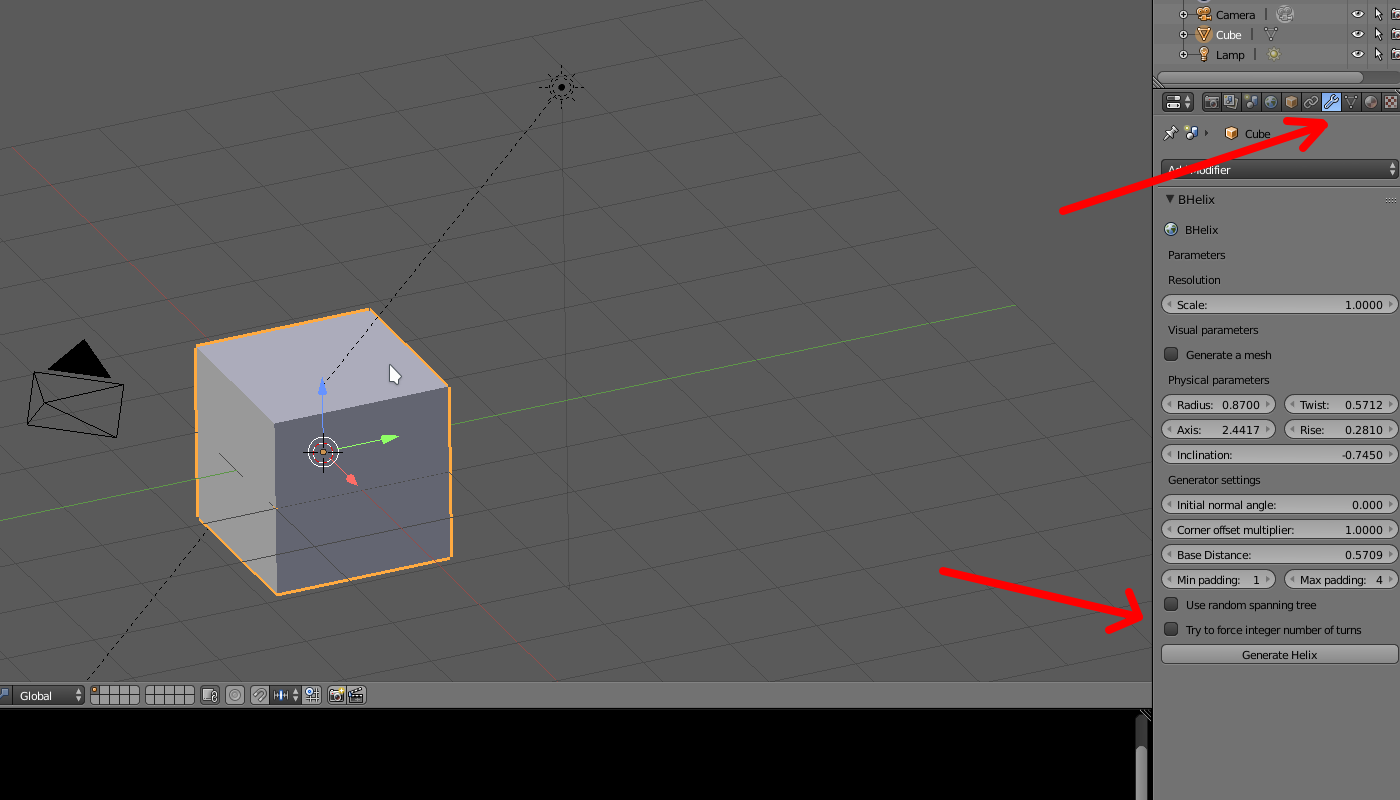
\includegraphics[width=\textwidth]{images/Sterna_5}
    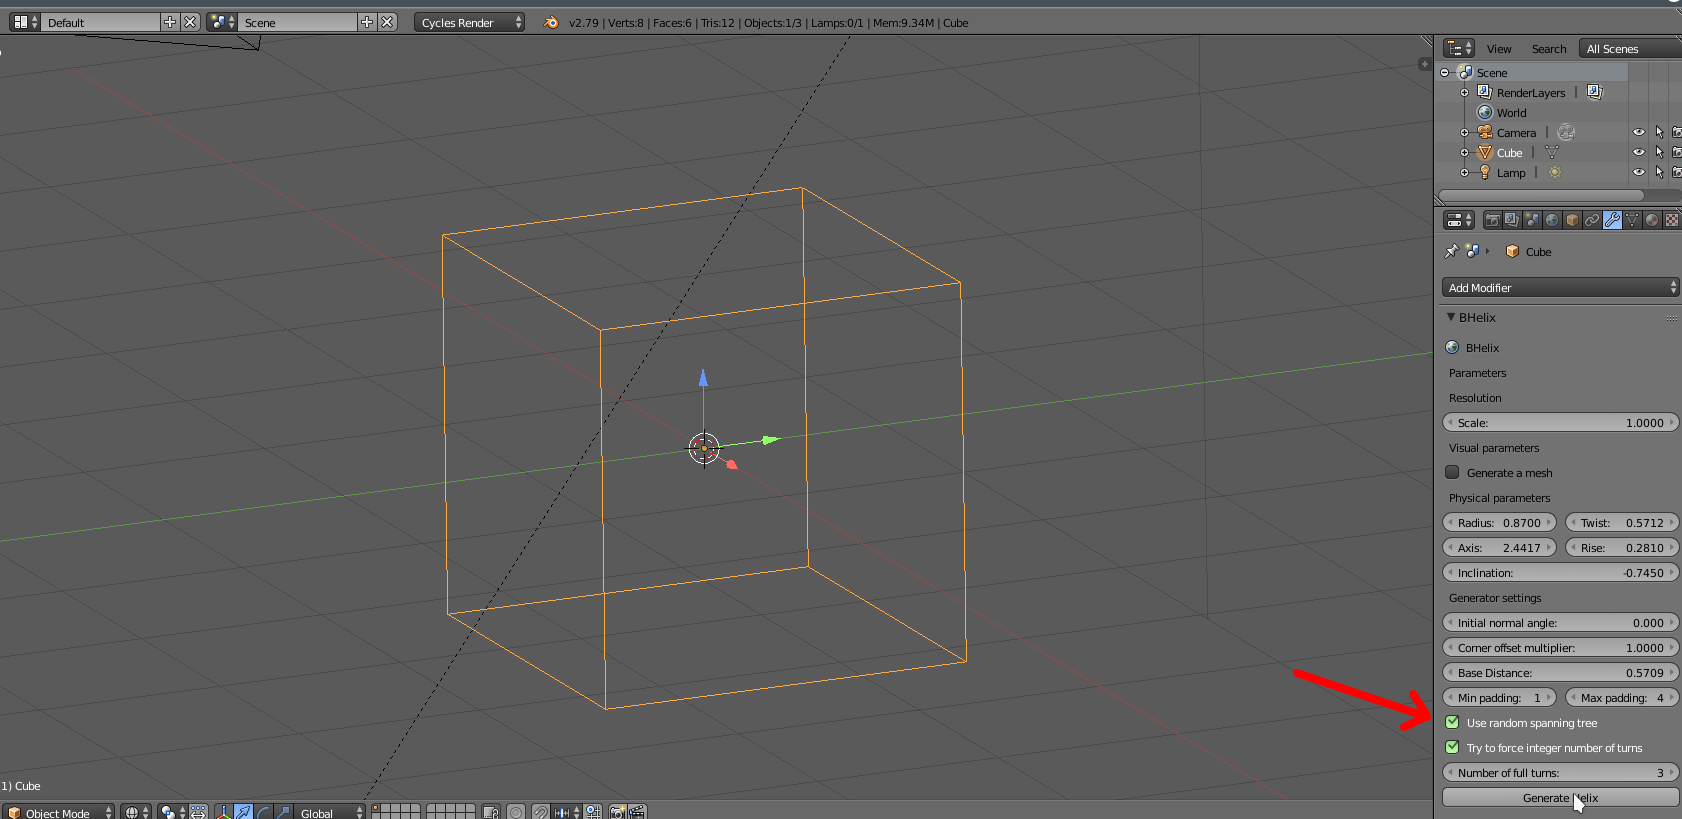
\includegraphics[width=\textwidth]{images/Sterna_7}
  \subsubsection{Input / Output}
    Sterna can import and export RNA strands in SNAC fileformat. To export a SNAC file, navigate to \verb+File -> Exprot -> Snac+. Some attention should be paid to the options of the Sterna exporter. Generating UG pairs and their proportion in a helix can be toggled and changed, descriptive comments can be added and linkers can be replaced by any bases. If you wish to simulate the RNA strand with OxRNA, for instance, make sure "Add promoter sequences" is not ticked, since it adds 35 extra bases at the origin.
    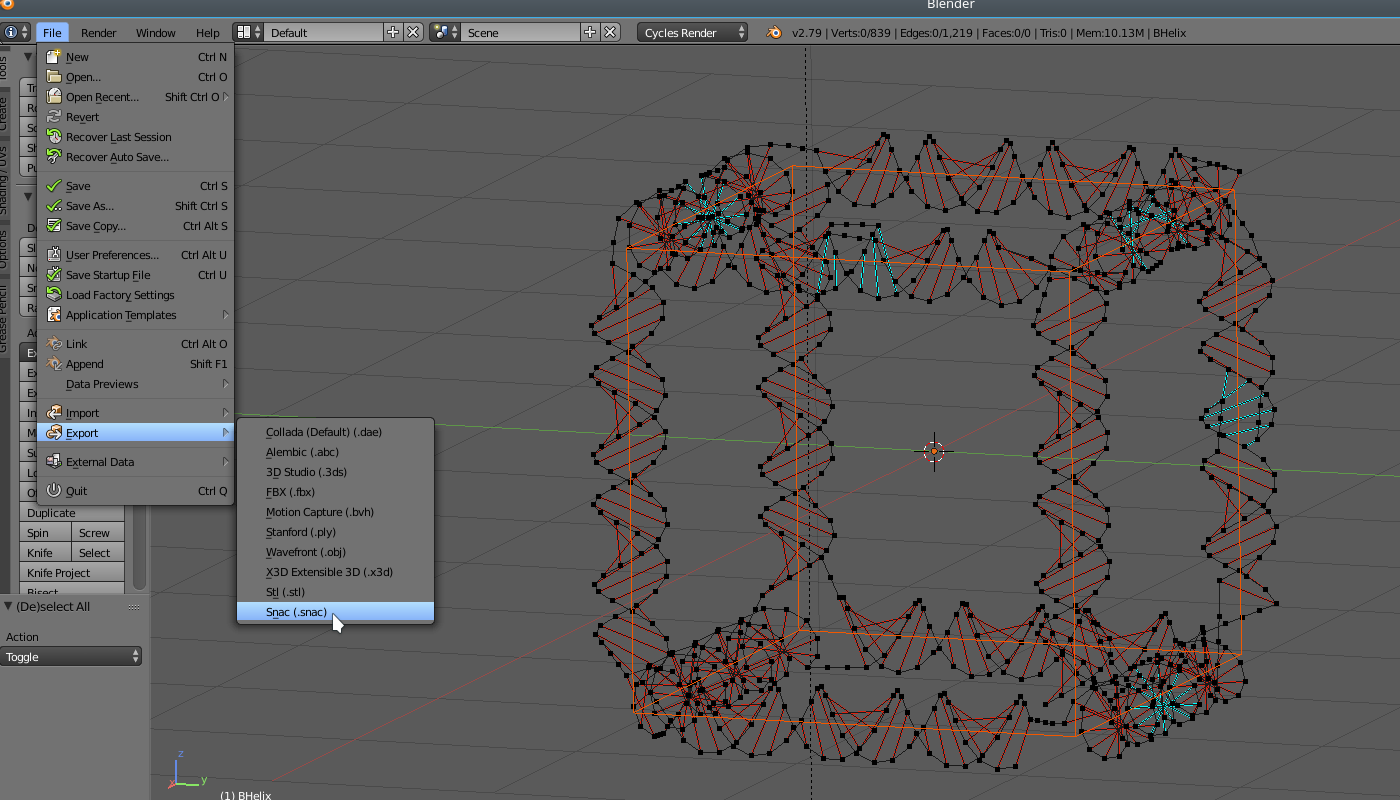
\includegraphics[width=\textwidth]{images/Sterna_8}
    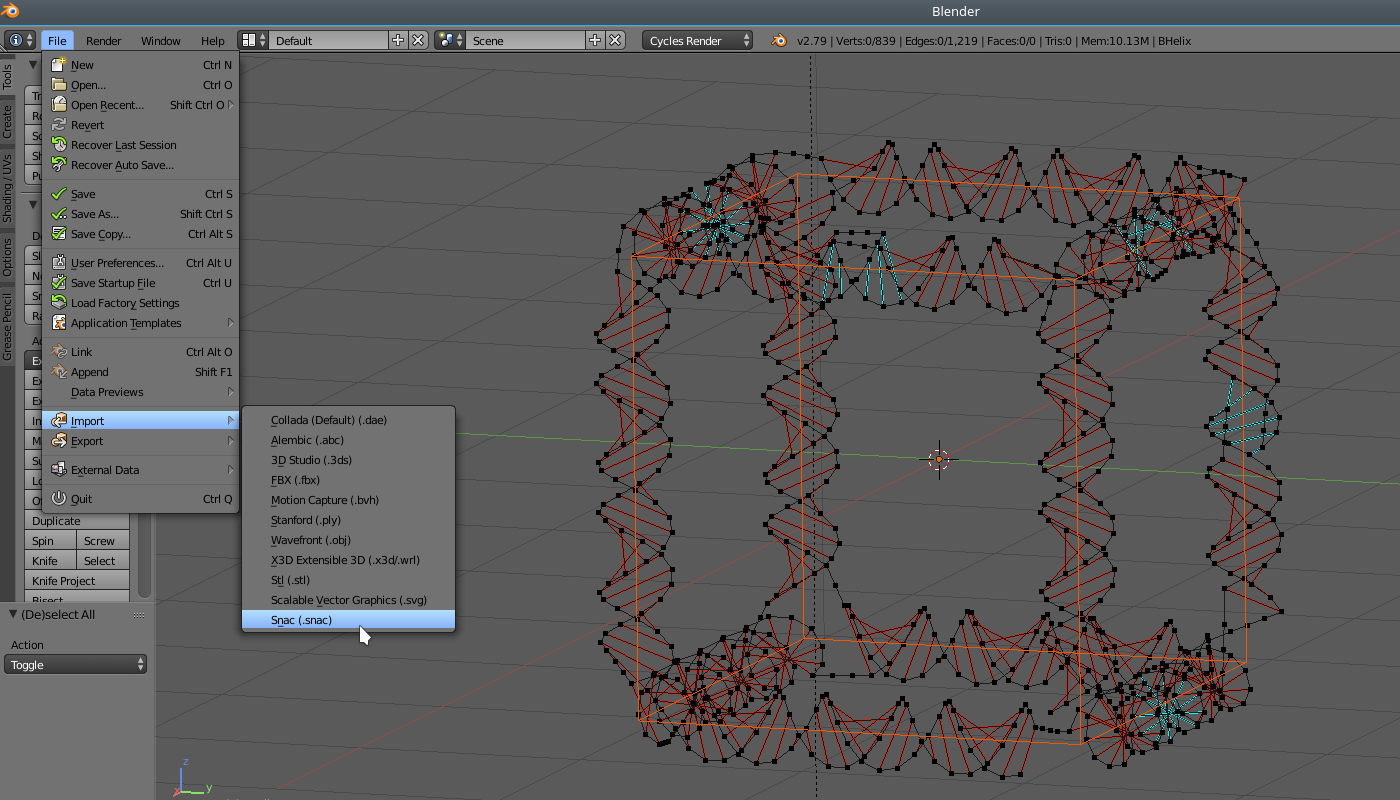
\includegraphics[width=\textwidth]{images/Sterna_9}
    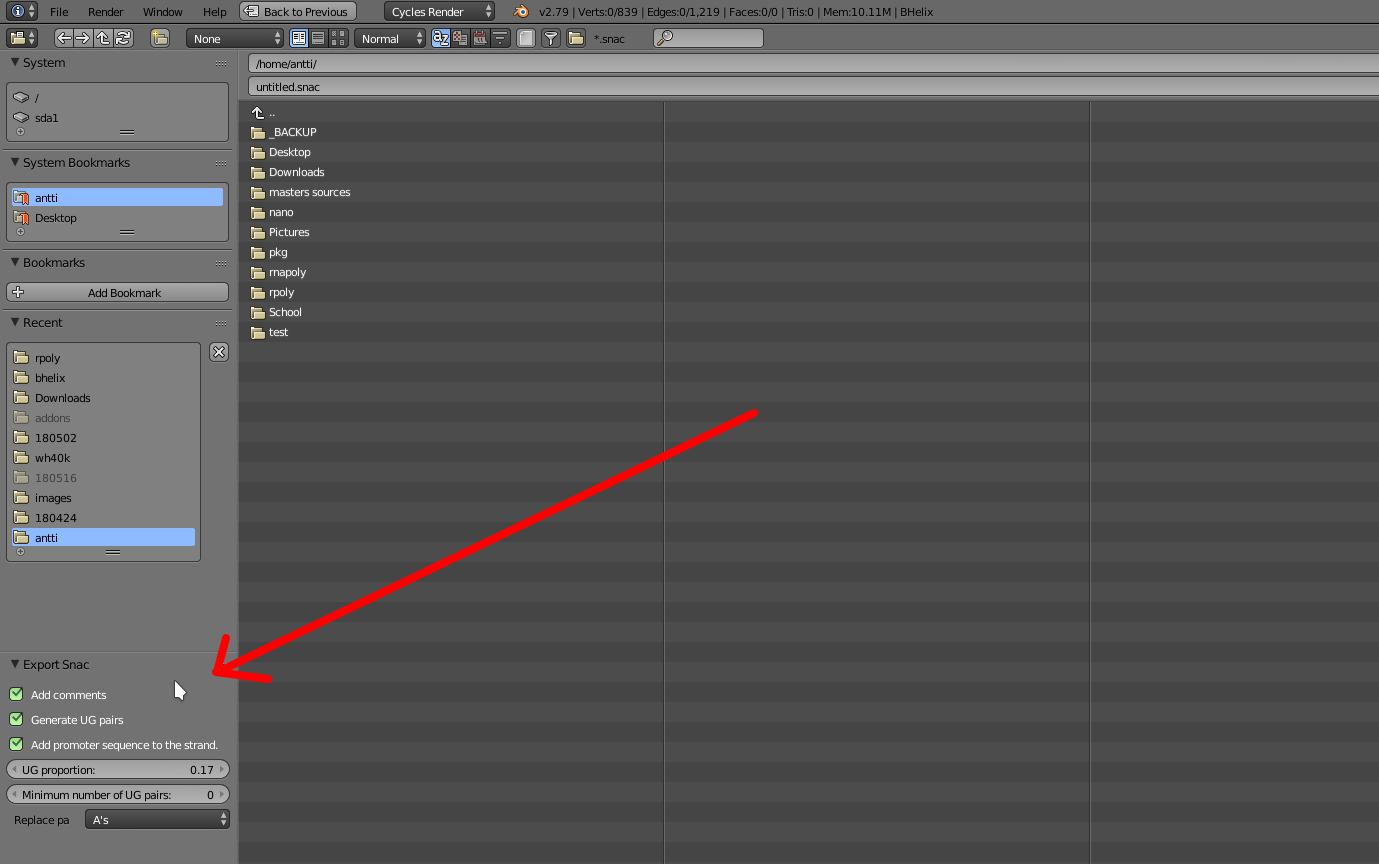
\includegraphics[width=\textwidth]{images/Sterna_10}
  \subsection{Settings}
    Sterna strand generation is affected by numerous input parameters and switches. What follows is a list explaining all of them.
    \begin{itemize}
      \item Scale parameter defines the length of Blender units in nanometers. A scale of 10 would mean that an edge of width 3.0 would be 30 nanometers long.
      \item Radius is a P-sticks model parameter, which defines the radius of the cylinder upon which bases are placed. A-form helix radius is 0.87 nm.
      \item Twist is a P-sticks model parameter, which defines the angle between consecutive bases along the helical axis. A-form helix twist is 0.5712 radians.
      \item Axis is a P-sticks model parameter, which defines the angle between bases from 5'-3' and from 3'-5' directions. A-form helix axis is 2.4417 radians.
      \item Rise is a P-sticks model parameter, which defines the distance between two consecutive bases along the helical axis. A-form helix rise is 0.2810 nm.
      \item Inclination is a P-sticks model parameter which defines the distance between two paired bases along the helical axis. A-form helix inclination is -0.745 nm, 5'-side ahead of 3'-side.
      \item Corner offset multiplier defines how close two helices are allowed to come to each other at vertices. A value of 0 would allow full overlap, a value of 1.0 zero overlap.
      \item Base distance defines the distance between two consecutive bases. It affects the density of linkers between helices.
      \item Min padding defines the minimum number of linkers between two helices.
      \item Max padding defines tha maximum number of linkers between two helices.
      \item Use adaptive offset switch forces the helices to get as close to each other as possible at vertices. If not toggled, all helices will be equidistant from the vertex.
      \item Use random spanning tree switch routes the helix around a random spanning tree instead of a user-defined spanning tree.
      \item Try to force integer number of turns switch tries to maximize the number of edges with integer number of full turns by modifying the scale parameter.
      \item Number of fulls defines how many turns the integer length edges should have.
      \item Spring relax switch tries to orientate the helices in a way which minimizes the distances/number of linkers between helices.
      \item Spring order defines the order of the spring strength. Larger values weigh long distance more strongly.
      \item Relaxation steps defines how many iterations the spring relaxation algorithm should perform. Larger values take longer but produce better results.
    \end{itemize}
